\documentclass{report}
\usepackage{fancyhdr} % Required for custom headers
\usepackage{lastpage} % Required to determine the last page for the footer
\usepackage{extramarks} % Required for headers and footers
\usepackage{graphicx} % Required to insert images
%\usepackage{lipsum} % Used for inserting dummy 'Lorem ipsum' text into the template
\usepackage{amsmath}
\usepackage{float
}
\usepackage{graphicx} 
%\usepackage{amsfont}
%\usepackage{amssymb}

\usepackage{multicol}
% Margins
\topmargin=-0.5in
\evensidemargin=0in
\oddsidemargin=-0.5in
\textwidth=7.5in
\textheight=9.0in
\headsep=0.25in 


\pagestyle{fancy}

%\rhead{\textbf{Marshall's Recipes}} % Top right header
%\lhead{\textbf{Curry Stir Fry}}
%\chead{ }
%\title{Curry Stir Fry}

\begin{document}
%\vspace{8mm}
%\textbf{PRELIMINARIES:}


\bigskip

\bigskip

\begin{multicols}{2}
\textbf{Ingredients}
\begin{itemize}
\item 2 lbs ground beef \quad (1935 kCal/ 171 gP/ 135 gF/ 0 gC)
\item 1 yellow onion \quad (45 kCal/ 1 gP/ 0 gF/ 11 gC)
\item about 6 ribs of celery \quad (45 kCal/ 2 gP/ 0 gF/ 11 gC)
\item 2 red bell peppers  \quad (36 kCal/ 2 gP/ 0 gF/ 8 gC)
\item 1 can pinto beans \quad (385 kCal/ 21 gP/ 3 gF/ 70 gC)
\item 2 cans kidney beans \quad (910 kCal/ 56 gP/ 8 gF/ 168 gC)
\item 1 can fire roasted tomatoes \newline   (105 kCal/ 4 gP/ 0 gF/ 21 gC)
\item 2 8 oz. cans tomato sauce \newline (106 kCal / 8 gP / 0 gF / 22 gC)
\item A fuckton of minced garlic
\item 2 tbsp. cumin
\item 1 tbsp. red pepper flakes
\item 4 tbsp. chili powder
\item 1 tsp. cayenne pepper
\item 2 tsp. salt
\item 1 tsp. smoked paprika
\item 1 cup water 



\end{itemize}


\columnbreak
\textbf{Procedure:}

\begin{enumerate}
\item \textit{\textbf{Note:}} Trust me on the celery. Sounds weird, but it adds a really nice crunchy texture to the chili and it's a good way to get the extra veggies in! A can of corn isn't bad to add in either, if you're feeling adventurous.
\item Cook ground meat with onion and bell peppers. 

\item Drain excess grease and add tomatoes, seasonings, and water. Bring to a boil. 

\item Add beans, cover and simmer for 1-2 hours. 

\item Serve with shredded cheese on top. Colby jack is my favorite! Highly recommend serving over fritos but it's not the healthiest. 
\end{enumerate}

\begin{table}[H]
  \begin{center}
    \caption{Macro totals}
    \label{tab:table1}
    \begin{tabular}{c|c|c|c} % <-- Alignments: 1st column left, 2nd middle and 3rd right, with vertical lines in between
      \textbf{Calories} & \textbf{Protein} & \textbf{Fat} & \textbf{Carbs}\\
      \hline
      3,567 kCal & 265 g & 146 g & 311 g\\
    \end{tabular}
  \end{center}
\end{table}
\end{multicols}




%\begin{center}
%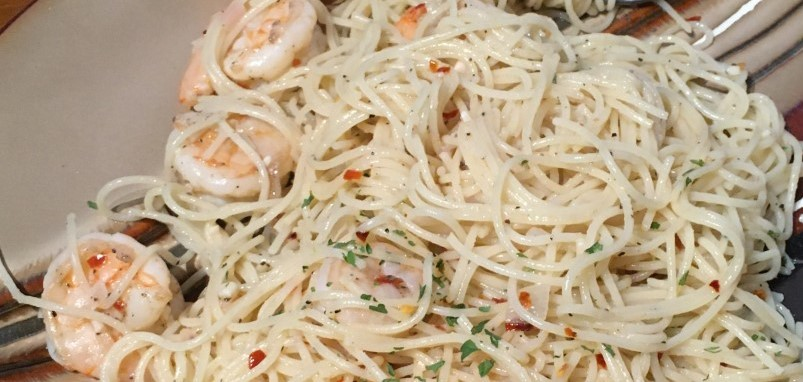
\includegraphics[scale=0.65]{Pasta/Shrimp Scampi/Shrimp Scampi.jpg}
%\end{center}


\end{document}